\section{Technischer Feasibility Check}
Der automatisierte technische Feasibility Check, bezeichnet eine ''Machbarkeitsprüfung'' oder ''Machbarkeitsstudie'', die bewertet, ob ein Stresstest an einem \gls{RPT}-Laborstandort durchgeführt werden kann.

Der Check ist ein integraler Bestandteil des \gls{REALIS}-\nameref{Subsec:project-lifecycle}, wie in Kapitel \ref{Subsec:project-lifecycle} beschrieben. Derzeit wird dieser manuell von Mitarbeitern des \gls{RPT}-Labors durchgeführt und in \gls{REALIS} dokumentiert. Dafür prüfen sie, ob die im Labor vorhandenen Kapazitäten und Bedingungen ausreichen, um die geforderten Tests für das jeweilige Produkt durchzuführen.

Die Beurteilung basiert auf mehreren Parametern. Um diese besser zu verstehen, wird im folgenden Kapitel erläutert, wie ein Stresstest im Detail abläuft und welche Schritte dabei erforderlich sind.


\subsection{Stresstests (Reliability Tests)}

Stresstests, auch als \textit{Reliability Tests} bezeichnet, sind ein wesentlicher Bestandteil der Qualifikation neuer Produkte. Sie prüfen die Belastbarkeit und Zuverlässigkeit unter definierten Bedingungen indem sie einen künstlichen Alterungsprozess simulieren. So lässt sich sicherstellen, dass die Chips über ihre gesamte Lebendauer hinweg einwandfrei funktionieren. Die häufigsten Testparameter sind dabei Temperatur (Hitze- und Kälte), Druck, Feuchtigkeit. Zusätzlich gibt es auch mechanische oder elektrische Belastungen, wobei auch Kombinationen dieser Umgebungsbedingungen/Belastungen eingesetzt werden.

Jeder Stresstest setzt sich aus mehreren aufeinanderfolgenden Operationen zusammen, die von einem \gls{RPT}-Labor-\gls{operator} mithilfe eines Test-\glspl{los}s (einer kleinen Stückzahl des Produkts) durchgeführt werden. Üblicherweise beginnt ein Test mit einer ''START''-Operation und endet mit einer ''END''-Operation. Dazwischen erfolgen mehrere Stressoperationen, die den spezifischen Stresstyp des Tests abbilden und die eigentliche Belastungsprüfung darstellen. Nach jeder Stressoperation wird das Los einer Funktionsprüfung (weitere Operation) unterzogen, um sicherzustellen, dass alle Chips die vorhergehende Belastung unbeschadet überstanden haben.

Während der Durchführung der Stressoperationen platziert der \gls{operator} das \gls{los} in einer geeigneten Testmaschine und passt die Parameter gemäß den geplanten Vorgaben in \gls{REALIS} an. Dabei kann eine Operation mehrere verschiedene Parameter mit vordefinierten Werten enthalten. Beispielsweise wird bei Temperaturtests die Zieltemperatur sowie die Testdauer eingestellt, während bei anderen Tests, wie etwa mechanischen Belastungen, die Anzahl der Wiederholungen definiert wird. Die Chips des Loses werden dabei häufig auf einem sogenannten \gls{board} montiert, das als Träger fungiert und Leiterbahnen enthält, um die elektrische Verbindung zwischen dem Testsystem und den Chips herzustellen.

\begin{figure}[!htbp]
    \centering
    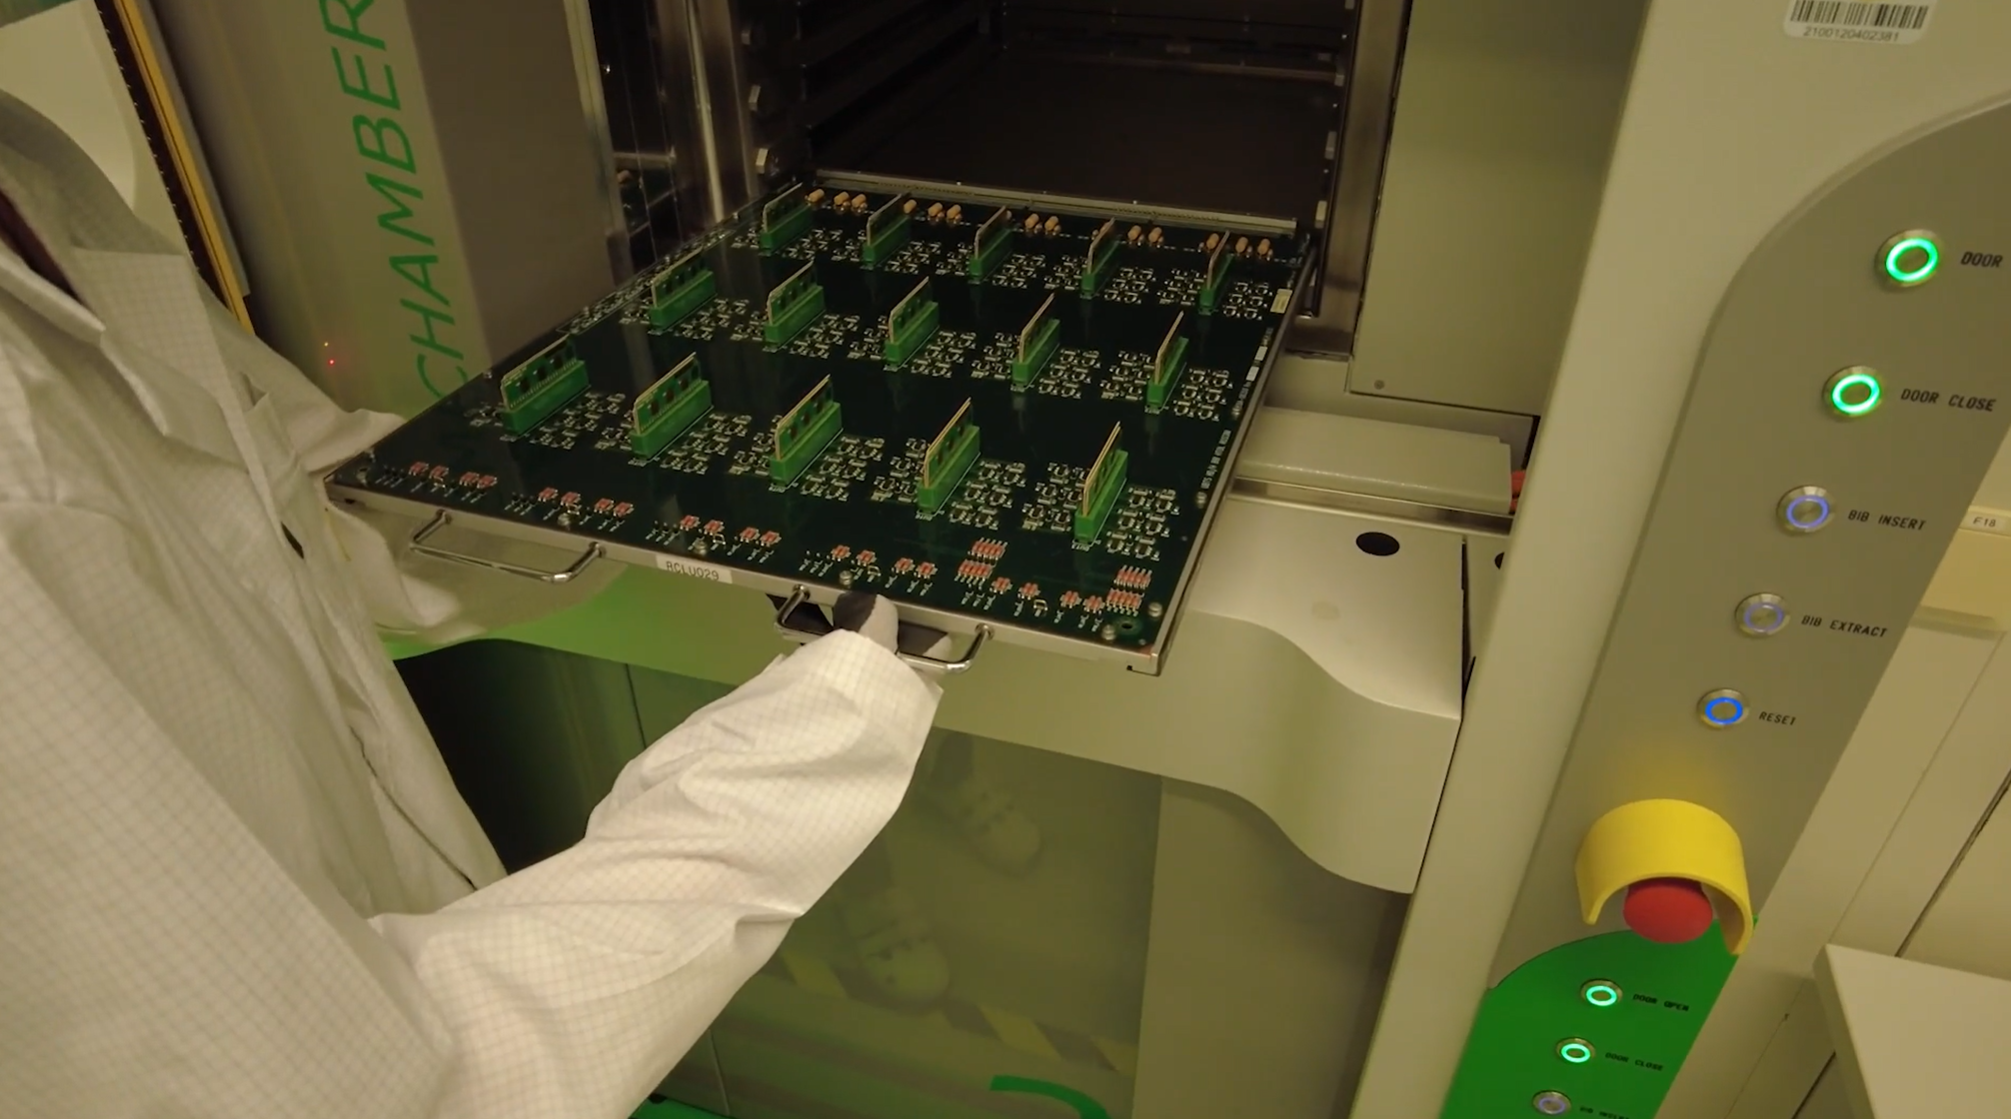
\includegraphics[width=0.95\textwidth]{bilder/testmaschine-with-board-substrate.png}
    \caption{Testmaschine mit Board (große grüne Platte), Substraten (kleine senkrechten eingesteckte Plättchen auf Board) und Chips \cite{RPTLaborIntern}}
    \label{fig:testmachine-with-board-substrate}
\end{figure}

Für kleinere Chips kommt oft ein zusätzliches Zwischenelement, das sogenannte \gls{substrate}, zum Einsatz. Das \gls{substrate} fungiert als Trägerelement und enthält ebenfalls Leiterbahnen. Es dient dazu, die Kontakte des Chips zu „vergrößern“ und somit die Handhabung und Verbindung mit dem \gls{board} zu erleichtern.
In Abbildung \ref{fig:testmachine-with-board-substrate} ist ein \gls{RPT}-Labor \gls{operator} zu sehen, der ein Board mit Substraten, auf denen die kleinen Chips sind, in eine Testmaschine schiebt.


In einigen Testverfahren, wie beispielsweise in Regensburg, wird jedoch kein \gls{board} benötigt. Hier werden die Chips in eine Karte (vergleichbar mit einer EC-Karte) integriert, die selbst als \gls{substrate} dient. Die Karte wird in einer Testmaschine wiederholt mechanischen Belastungen, wie Biegungen, ausgesetzt, wie in Abbildung \ref{fig:stresstest-card}. Die Karten werden dabei einzeln in die Maschine eingelegt, was den Einsatz eines \glspl{board} überflüssig macht.

\begin{figure}[!htbp]
    \centering
    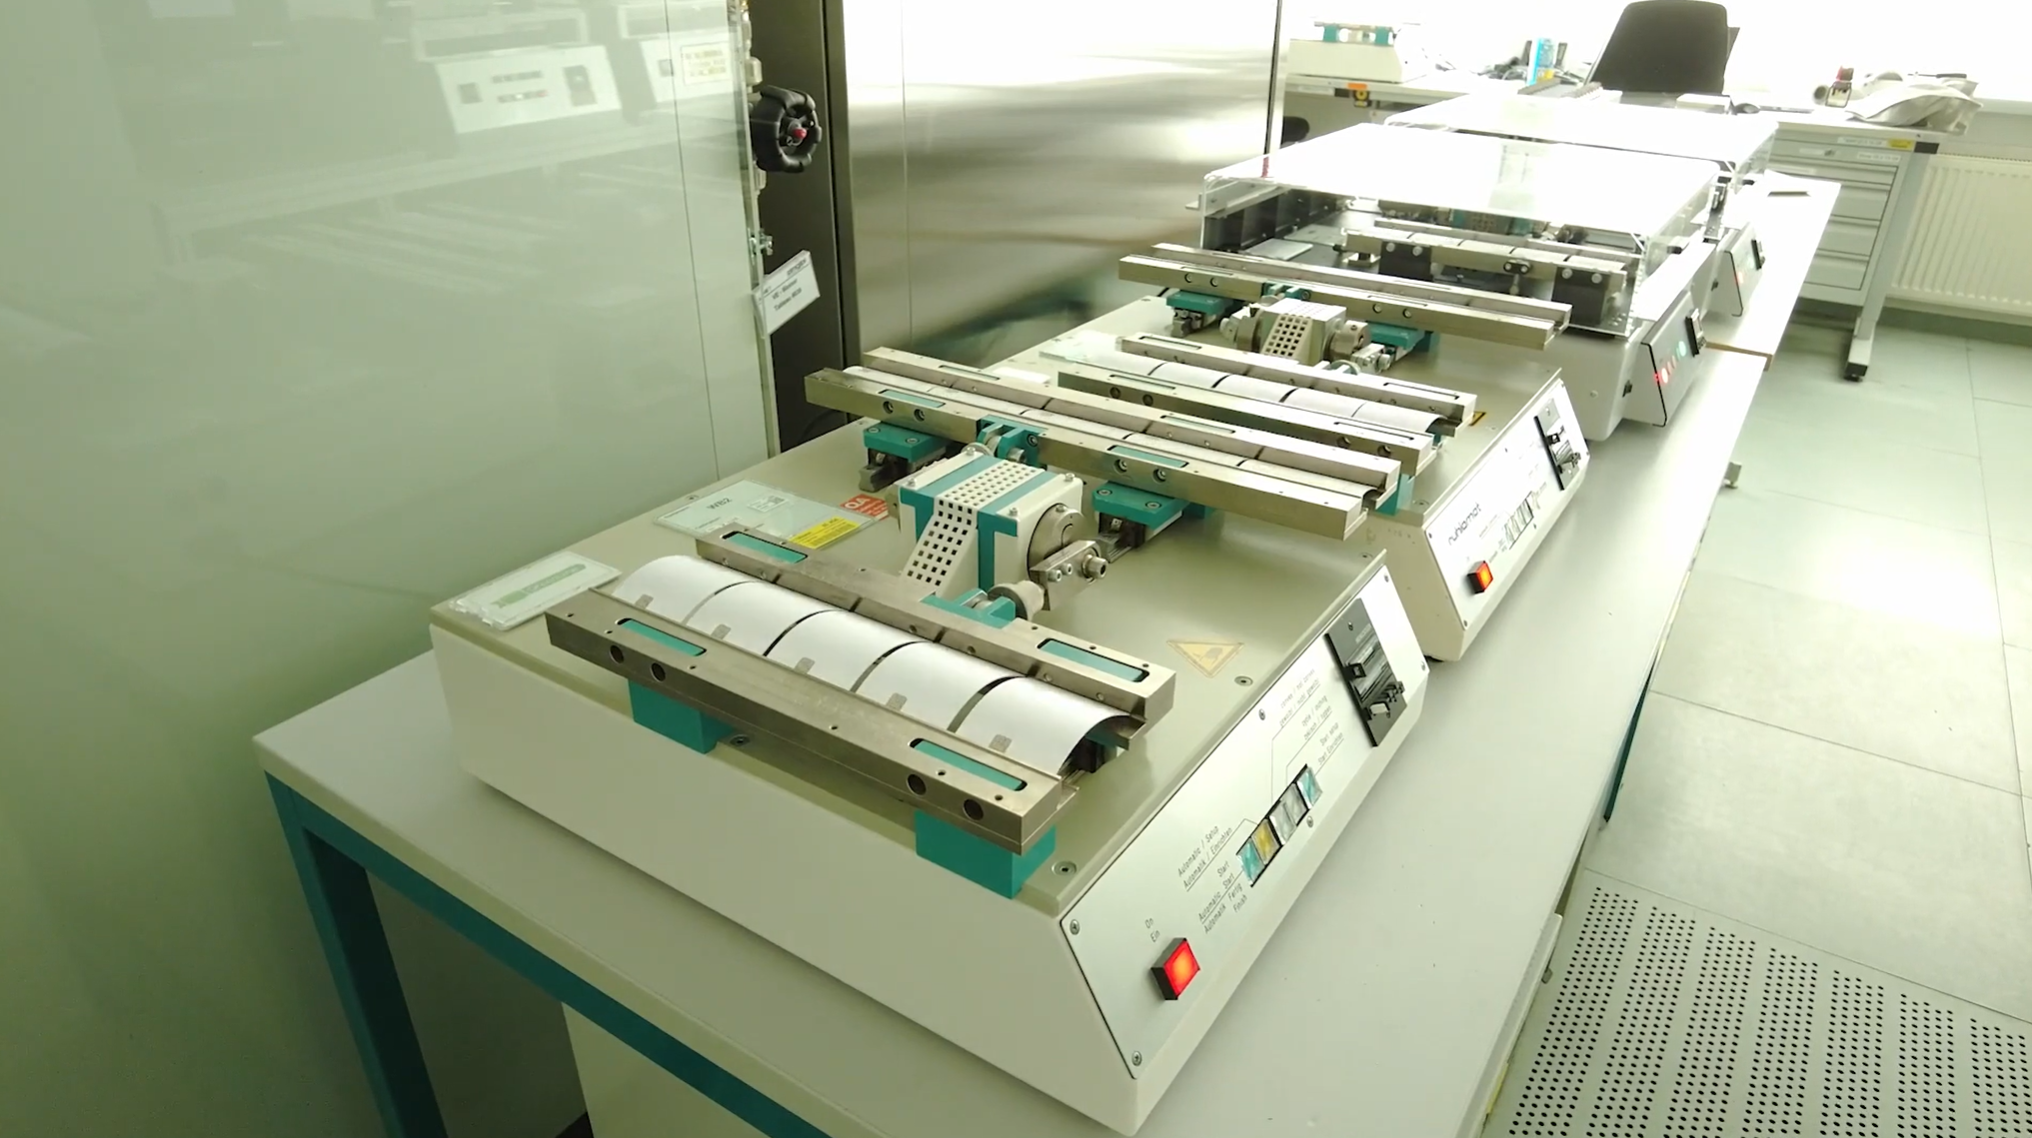
\includegraphics[width=1\textwidth]{bilder/stresstest-card1.png}
    \caption{Biege-Stresstest mit Karten \cite{RPTLaborIntern}}
    \label{fig:stresstest-card}
\end{figure}

Alle durchgeführten Operationen eines Tests müssen vom \gls{operator} in \gls{REALIS} dokumentiert werden, insbesondere die Stressoperationen und die anschließenden Funktionsprüfungen. Dabei werden unter anderem die Anzahl der Chips, die nach einer Stressoperation ausgefallen sind, sowie die vermuteten Ursachen des Ausfalls festgehalten.
Nur wenn das gesamte \gls{los} unbeschadet ist kann mit der nächsten Operation fortgefahren werden, ansonsten wir der Test vorerst gestoppt und der \gls{QM} muss entscheiden, wie weiter vorgegangen wird.

\subsection{Parameter des technischen Feasibility Checks}\label{Subsec:ParameterdestechnischenFeasibilityChecks}

Im Rahmen des technischen Feasibility Checks wird zunächst geprüft, ob die vom \gls{QM} definierten Parameter und Werte der geplanten Stressoperationen sinnvoll und durchführbar sind. Dies umfasst beispielsweise die Überprüfung, ob die vorgegebene Testtemperatur im technisch möglichen Bereich liegt. Zudem wird kontrolliert, ob für jeden Parameter ein geeigneter Wert festgelegt wurde, falls dies erforderlich ist. Diese Überprüfung wird in dieser Arbeit auch mit dem Begriff \textbf{\gls{ConditionCheck}} beschrieben.

Anschließend wird geprüft, ob am zuständigen \gls{RPT}-Labor geeignete Stressmaschinen für den geforderten Stresstesttyp verfügbar sind. Dabei wird sichergestellt, dass die Maschinen einsatzbereit, nicht defekt und auch nicht in Wartung sind. Außerdem wird überprüft, ob sie die vorgegebenen Parameter und Werte tatsächlich umsetzen können. Diese Überprüfungen werden in der Arbeit auch mit dem Begriff \textbf{\gls{EquipmentCheck}} bezeichnet.
Zusätzlich wird kontrolliert, ob passende \glspl{board} und \glspl{substrate} für die Chips des \glspl{los}s vorhanden sind, sofern diese benötigt werden.\todo{wird hier aber nicht mehr umgesetzt}

Aktuell muss ein Mitarbeiter des Labors all diese Prüfungen für jeden Stresstest manuell durchführen. Bei wiederkehrenden Tests kann es sein, dass der Mitarbeiter bereits aus Erfahrung weiß, dass der Test durchführbar ist, und der Feasibility Check somit direkt im System bestätigt werden kann. In anderen Fällen kann es jedoch mehrere Stunden dauern, um die Machbarkeit eines Tests festzustellen.

Um diesen Prozess zu beschleunigen und eine höhere Effizienz zu erreichen, soll dieser Schritt des \nameref{Subsec:project-lifecycle} von \gls{REALIS} automatisiert werden. Wie genau diese Automatisierung umgesetzt werden soll, wird im nächsten Kapitel (\nameref{Chap:Anforderungen}) beschrieben.
